% ----- formatovani dokumentu -----------------------------------------------
\documentclass[12pt,a4paper,titlepage,final]{report}
\usepackage[utf8]{inputenc}
\usepackage[T1, IL2]{fontenc}
\usepackage{graphicx}
\usepackage{epstopdf}
\usepackage[margin=2cm]{caption}
\usepackage[top=3cm, left=2cm, right=2cm, text={17cm, 24cm}, ignorefoot]{geometry}
\usepackage{color}
\usepackage{url}
\usepackage{setspace}
\singlespacing
\usepackage[square, numbers]{natbib}
\pagestyle{plain}
\pagenumbering{arabic}
\setcounter{page}{1}
\setcounter{secnumdepth}{-1}
\setlength{\parindent}{1cm}
\usepackage{natbib}


% ----- vyberte jazyk -------------------------------------------------------
\usepackage[english,czech]{babel}
%\usepackage[english]{babel}

% ----- dopiste titulky -----------------------------------------------------
\newcommand\Course{Počítačová grafika}
\newcommand\WorkTitle{Realistické generování oblohy}
\newcommand\AuthorA{Miloslav Číž}
\newcommand\AuthorAEmail{xcizmi00@stud.fit.vutbr.cz}
\newcommand\AuthorB{Aleš Dujíček}
\newcommand\AuthorBEmail{xdujic01@stud.fit.vutbr.cz}
\newcommand\Faculty{Fakulta Informačních Technologií}
\newcommand\School{Vysoké Učení Technické v Brně}

\usepackage[
pdftitle={\WorkTitle},
pdfauthor={\AuthorA, \AuthorB},
bookmarks=true,
colorlinks=true,
breaklinks=true,
urlcolor=blue,
citecolor=blue,
linkcolor=blue,
unicode=true,
]
{hyperref}


% ----- titulni strana ------------------------------------------------------

\begin{document}
    \begin{titlepage}
    \begin{center}
        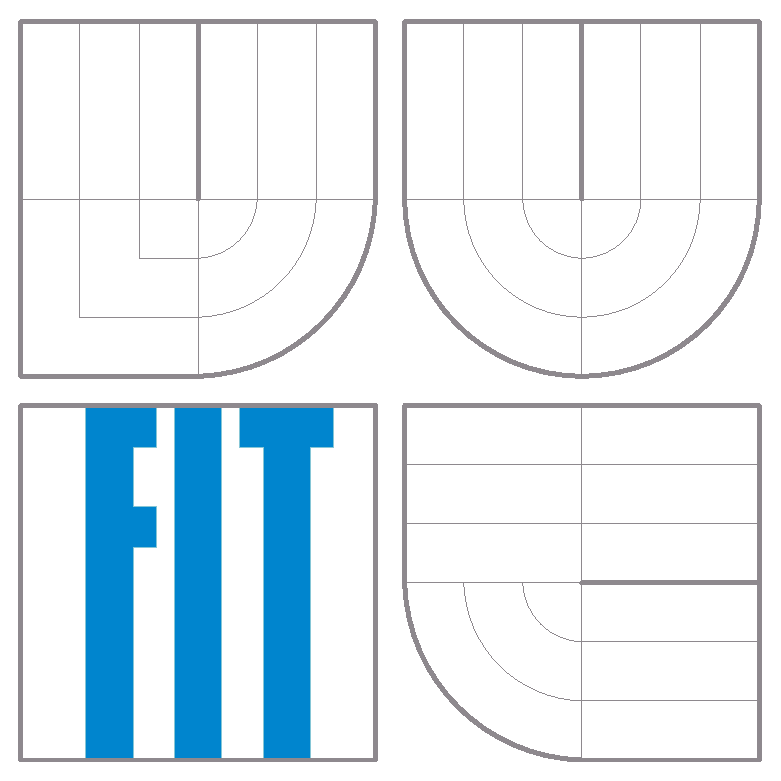
\includegraphics[height=5cm]{images/logo.eps}
    \end{center}
    \vfill
    \begin{center}
        \begin{Large}
            \Course\\
        \end{Large}
        \bigskip
        \begin{Huge}
            \WorkTitle\\
        \end{Huge}
    \end{center}
    \vfill
    \begin{center}
        \begin{large}
            \today
        \end{large}
    \end{center}
    \vfill
    \begin{flushleft}
        \begin{large}
            \begin{tabular}{lll}
                Autoři: & \AuthorA, & \url{\AuthorAEmail} \\
                        & \AuthorB, & \url{\AuthorBEmail} \\
                & & \\
                & \Faculty \\
                & \School \\
            \end{tabular}
        \end{large}
    \end{flushleft}
\end{titlepage}

% ----- obsah --------------------------------------------------------------

\tableofcontents

% ----- zadani -------------------------------------------------------------
\newpage
\chapter{Zadání}

Zadáním bylo vytvořit program pro vhodně parametrizovatelné generování realistických obrázků oblohy za použití vhodné metody (založené např. na sledování paprsku). Měli jsme se zaměřit na vizuální kvalitu oblohy, krajinu stačilo vykreslit pouze velmi zjednodušeně. Zadání jsme upřesnili následujícím způsobem:

\begin{itemize}
    \item generování obrázků oblohy podobných fotografii
    \item metoda: sledování paprsku v kombinaci s 2D vykreslováním
    \item procedurální generování textury mraků
    \item možnost generovat sekvenci obrázků jako animaci (volitelně navazující)
\end{itemize}

%---------------------------------------------------------------------------
\chapter{Nejdůležitější dosažené výsledky}

Popište 3 věci, které jsou na vašem projektu nejlepší. Nejlépe ukažte a
komentujte obrázky, v nejhorším případě vypište textově.

\section{Plynulá animace}

Náš program umožňuje nad rámec zadání generovat animaci oblohy, která
může být buď mezi dvěma časovými úseky během dne, anebo během jednoho
časového okamžiku -- animace potom ve smyčce spojitě navazuje díky
spojitosti implementovaného 3D šumu.

\begin{itemize}
    \item Položka 1
    \begin{itemize}
        \item Podpoložka 1.1
        \item Podpoložka 1.2
        \item $\ldots$
    \end{itemize}
    \item Položka 2
    \item $\ldots$
\end{itemize}

\begin{center}
    \captionsetup{type=figure}
        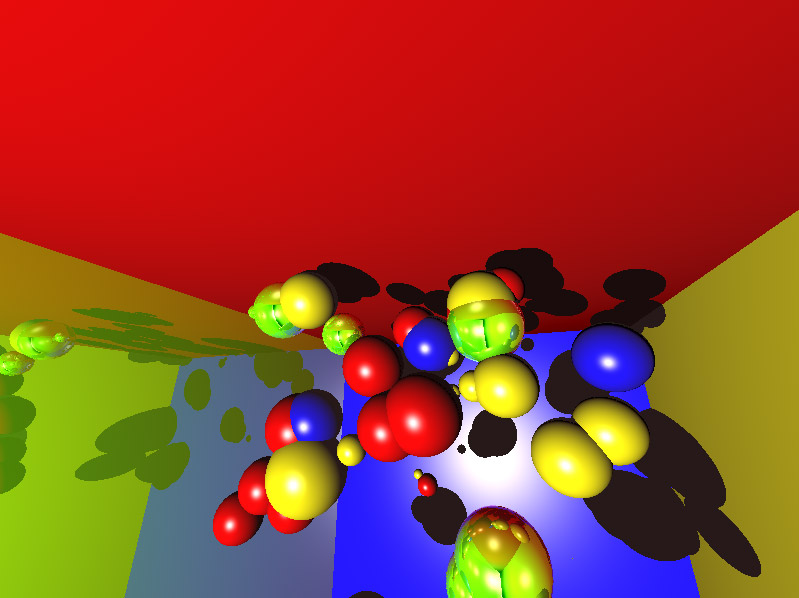
\includegraphics[width=10cm]{images/sample.jpg}
    \captionof{figure}{Popisek vzorového obrázek}
\end{center}

\section{Paralelizace}

možná nějaký odhad zrychlení

\begin{table}[h!]
    \begin{center}
    \begin{tabular}{ | p{3.5cm} | p{3.5cm} | p{3.5cm} | p{3.5cm} |}
    \hline
    Sloupec A & Sloupec B & Sloupec C & Sloupec D
    \\ \hline

    A1 & B1 & C1 & D1
    \\ \hline

    A2 & B2 & C2 & D2
    \\ \hline

    \end{tabular}
    \end{center}
    \caption{Vzorová tabulka}
\end{table}

\section{Třetí věc}

Vestibulum ac tellus et massa facilisis tristique in in ante. In elementum luctus ante, id cursus nulla. Quisque sit amet dolor dui. Suspendisse bibendum auctor augue, a posuere enim dictum non. Nunc iaculis libero eget interdum egestas. Suspendisse pretium cursus massa vel fringilla.



%---------------------------------------------------------------------------
\chapter{Zvláštní použité znalosti}

Uveďte informace, které byly potřeba nad rámec výuky probírané na FIT.
Vysvětlete je pomocí obrázků, schémat, vzorců apod.

3D perlinův šum, paralelizace

\paragraph{Rozsah:} podle potřeby a vlastního uvážení


%---------------------------------------------------------------------------
\chapter{Práce na projektu}

\begin{itemize}
\item \textbf{\AuthorA}: implementace sledování paprsku, vykreslení pozadí a~krajiny, hlavní program, dokumentace
\item \textbf{\AuthorB}: implementace Perlinova šumu, paralelizace
\end{itemize}

%---------------------------------------------------------------------------
\section{Co bylo nejpracnější}

\paragraph{Rozsah:} 5-10 řádků

\begin{itemize}
\item \textbf{\AuthorA}: Sestavit scénu a nastavit její parametry tak,
aby výstup alespoň trochu připomínal realitu.
\item \textbf{\AuthorB}:
\end{itemize}

%---------------------------------------------------------------------------
\section{Zkušenosti získané řešením projektu}

\begin{itemize}
\item \textbf{\AuthorA}: Poprvé jsem programoval ray-tracing -- naučil
jsem se základy matematiky, která se v~této oblasti
používá (barycentrické souřadnice, výpočty průsečíků apod.). Vyzkoušel
jsem si modelování reálné přírodní scény, což jsem dosud ve škole sám
nedělal.
\item \textbf{\AuthorB}:
\end{itemize}

\paragraph{Rozsah:} formulujte stručně, uchopte cca 3-5 věcí

%---------------------------------------------------------------------------
\chapter{Autoevaluace}

\paragraph{Technický návrh (85\%):}
Klíčové metody a~prostředky jsme si ujasnili před začátkem implementace
poté, co jsme projekt konzultovali. Některé věci, jako např.
supersampling, jsme přidávali až během implementace.

\paragraph{Programování (70\%):}
Kód jsme se snažili psát alespoň minimálně přehledně, objektově,
modulárně a~komentovat jej způsobem kompatibilním se systémy
pro automatické generování dokumentace. Bylo by možné
dosáhnout podstatně kvalitnějšího kódu, to však nebylo naším primárním
cílem.

\paragraph{Vzhled vytvořeného řešení (90\%):}
Vizuální výsledky hodnotíme s~ohledem na pracovní podmínky zdařile.
Nedokonalosti v~obrázcích jsou znát např. na mracích, pro lepší výsledky
by bylo možné použít lepší druh šumu (např. simplex noise).

\paragraph{Využití zdrojů (80\%):}
Využili jsme kód pro práci s~rastrovou grafikou a~formátem PNG napsaný v~rámci
bakalářské práce. Metody jsme zvolili na základě konzultace a~studia
literatury.

\paragraph{Hospodaření s časem (90\%):}
Pracovat jsme začali ihned po zadání, pokračovali jsme rovnoměrně.

\paragraph{Spolupráce v týmu (80\%):}
Snažili jsme se pracovat průběžně a práci každý týden konzultovat. Pro
správu kódu jsme využili systém GIT.

\paragraph{Celkový dojem (90\%):}
Zadání bylo podle nás z~programátorského hlediska průměrně náročné, ale
mělo navíc umělecký aspekt, se kterým se na škole příliš nesetkáváme,
proto jsme se díky projektu hodně naučili. Výsledný program je podle
nás použitelný v~jednoduché umělecké grafice, např. pro generování pozadí
pro videa apod.

%---------------------------------------------------------------------------
\chapter{Ovládání vytvořeného programu}

\section{Technologie potřebné pro spuštění programu}
Projekt využívá tyto technologie:

\begin{itemize}
\item jazyk C++
\item překladač gcc
\item knihovna LodePNG
\end{itemize}

Program je možné přeložit a~spustit na platformách, které mají C++
překladač.

\section{Obsluha programu}

Program se používá z~příkazové řádky následujícím způsobem:
{\tt skygen [[-t time][-d duration][-f frames][-o name][-c amount][-e density][-x width][-y height][-p level][-s] | [-h]]}

\begin{itemize}
\item {\tt -t} specifikuje denní dobu v~24hodinovém formátu {\tt HH:MM}.
\item {\tt -d} specifikuje trvání animace od dané denní doby celým číslem udávajícím počtet minut.
\item {\tt -f} udává počet snímků animace.
\item {\tt -o} říká, jaké bude jméno (jména) výstupního souboru.
\item {\tt -x} zadává šířku generovaného obrázku v~pixelech.
\item {\tt -y} zadává výšku generovaného obrázku v~pixelech.
\item {\tt -p} specifikuje stupeň supersamplingu.
\item {\tt -c} udává množství mraků celočíselnou hodnotou v~rozsahu 0 až 100.
\item {\tt -e} udává hustotu mraků celočíselnou hodnotou v~rozsahu 0 až 100.
\item {\tt -s} vypíná výpis zpráv během generování obrázků.
\item {\tt -h} zobrazí nápovědu.
\end{itemize}

%---------------------------------------------------------------------------
\chapter{Doporučení pro budoucí zadávání projektů}

Pozitivně hodnotíme volnost zadání projektů s~velkým prostorem pro
kreativitu a~možnost přihlásit se v~řípadě zájmu i~na téma, které je již
zabrané, čehož jsme sami využili.

%---------------------------------------------------------------------------

\bibliographystyle{plain}

\nocite{cite1}
\nocite{cite2}
\nocite{cite3}

\bibliography{reference}
\addcontentsline{toc}{chapter}{Literatura}

\end{document}

